\documentclass[aspectratio=169]{beamer}

% shift figures over so that they fit on the page
\usepackage{changepage}

% put line breaks in table cells
\usepackage{makecell}

% for making columns
\usepackage{multicol}

% include pretty pictures
\usepackage{graphicx}

% for giant question mark
\usepackage{anyfontsize}

% place captions beside figures
\usepackage{floatrow}


\usetheme{PaloAlto}
\usecolortheme{whale}

\title[]{Revamp of High Energy Physics Laboratory's Computer Systems}
\author[]{Josef Bostik \\Eric Pereira \\Ryan Wojtyla}
\date{February 15, 2019}

\begin{document}

%----------BEGIN TITLE----------

\begin{frame}
  \titlepage
\end{frame}

%-----------END TITLE-----------

%----------BEGIN GOALS----------

\section{Milestone 4 Goals}

\begin{frame}
  
  \frametitle{Milestone 4 Progress}

  \begin{center}
    \begin{tabular}{|c|c|c|c|c|c|}
      \hline
      Task & \% Completion & Eric & Josef & Ryan & To Do \\
      \hline
      \makecell{Integrate \\ cluster \\ components.} & 0\% & 0\% & 0\% & 0\% &
                                                                               \makecell{find
                                                                               new
                                                                               \\
      solutions}
      \\
      \hline
      \makecell{ Rewire the \\ existing MTS.} & 90\% & 70\% & 20\% & 0\% &
                                                            \makecell{miscellaneous \\ touch
                                                            ups} \\
      \hline
      \makecell{Resolve software \\ issues with \\ development MTS.} & 60\% & 0\% & 40\% & 20\% &
                                                                                 reinstall
                                                                                 AMORE
      \\
      \hline
    \end{tabular}
  \end{center}
  
\end{frame}

%-----------END GOALS-----------

%----------BEGIN GEM COMPUTERS----------

\section{GEM Computers}

\begin{frame}

  \frametitle{GEM Computers}

  \begin{itemize}
    \item Attempted to save Truth PC
    \item Checked computers RAID systems
    \item Adjusted drivers on multiple computers
    \item Assist GEM Team with programming issues. 
  \end{itemize}

\end{frame}

%-----------END GEM COMPUTERS-----------

%----------BEGIN CLUSTER----------

\section{Compute Cluster}

\begin{frame}

  \frametitle{Compute Cluster}

  \begin{multicols}{2}
    
    \begin{itemize}
      
    \item Ideally:
      \begin{enumerate}
      \item Node boots into ROCKS Kernel CD
      \item Node notifies head node of its existence
      \item Node requests kickstart file from head node
      \end{enumerate}
      
      \columnbreak
      
    \item In Reality:
      \begin{enumerate}
      \item Node boots into ROCKS Kernel CD
      \item Node notifies head node as soon as networking is enabled within
        the installer
      \item In what state does the node request a kickstart file?
      \end{enumerate}
      
    \end{itemize}
    
  \end{multicols}

  % see about throwing a picture of insert-ethers (maybe?) here

\end{frame}

%-----------END CLUSTER-----------

\section{Muon Tomography Station}

%----------BEGIN EXISTING MTS----------

\subsection{Existing MTS}

\begin{frame}

  \frametitle{Existing MTS}

  \begin{itemize}
    \item Cable lengths have been optimized
    \item Cables have been tidied up
    \item Obtained FEC firmware!
  \end{itemize}

%  \begin{figure}
%    \floatbox[{\capbeside\thisfloatsetup{
%        capbesideposition={right,top},capbesidewidth=4cm}}]
%    {figure}[\FBwidth]
%    {\caption{The unnecessarily long 20 foot cables connected the FECs and
%        computer to the network switches have been replaced with much more
%        appropriate 3 foot cables.}
%    }
%    {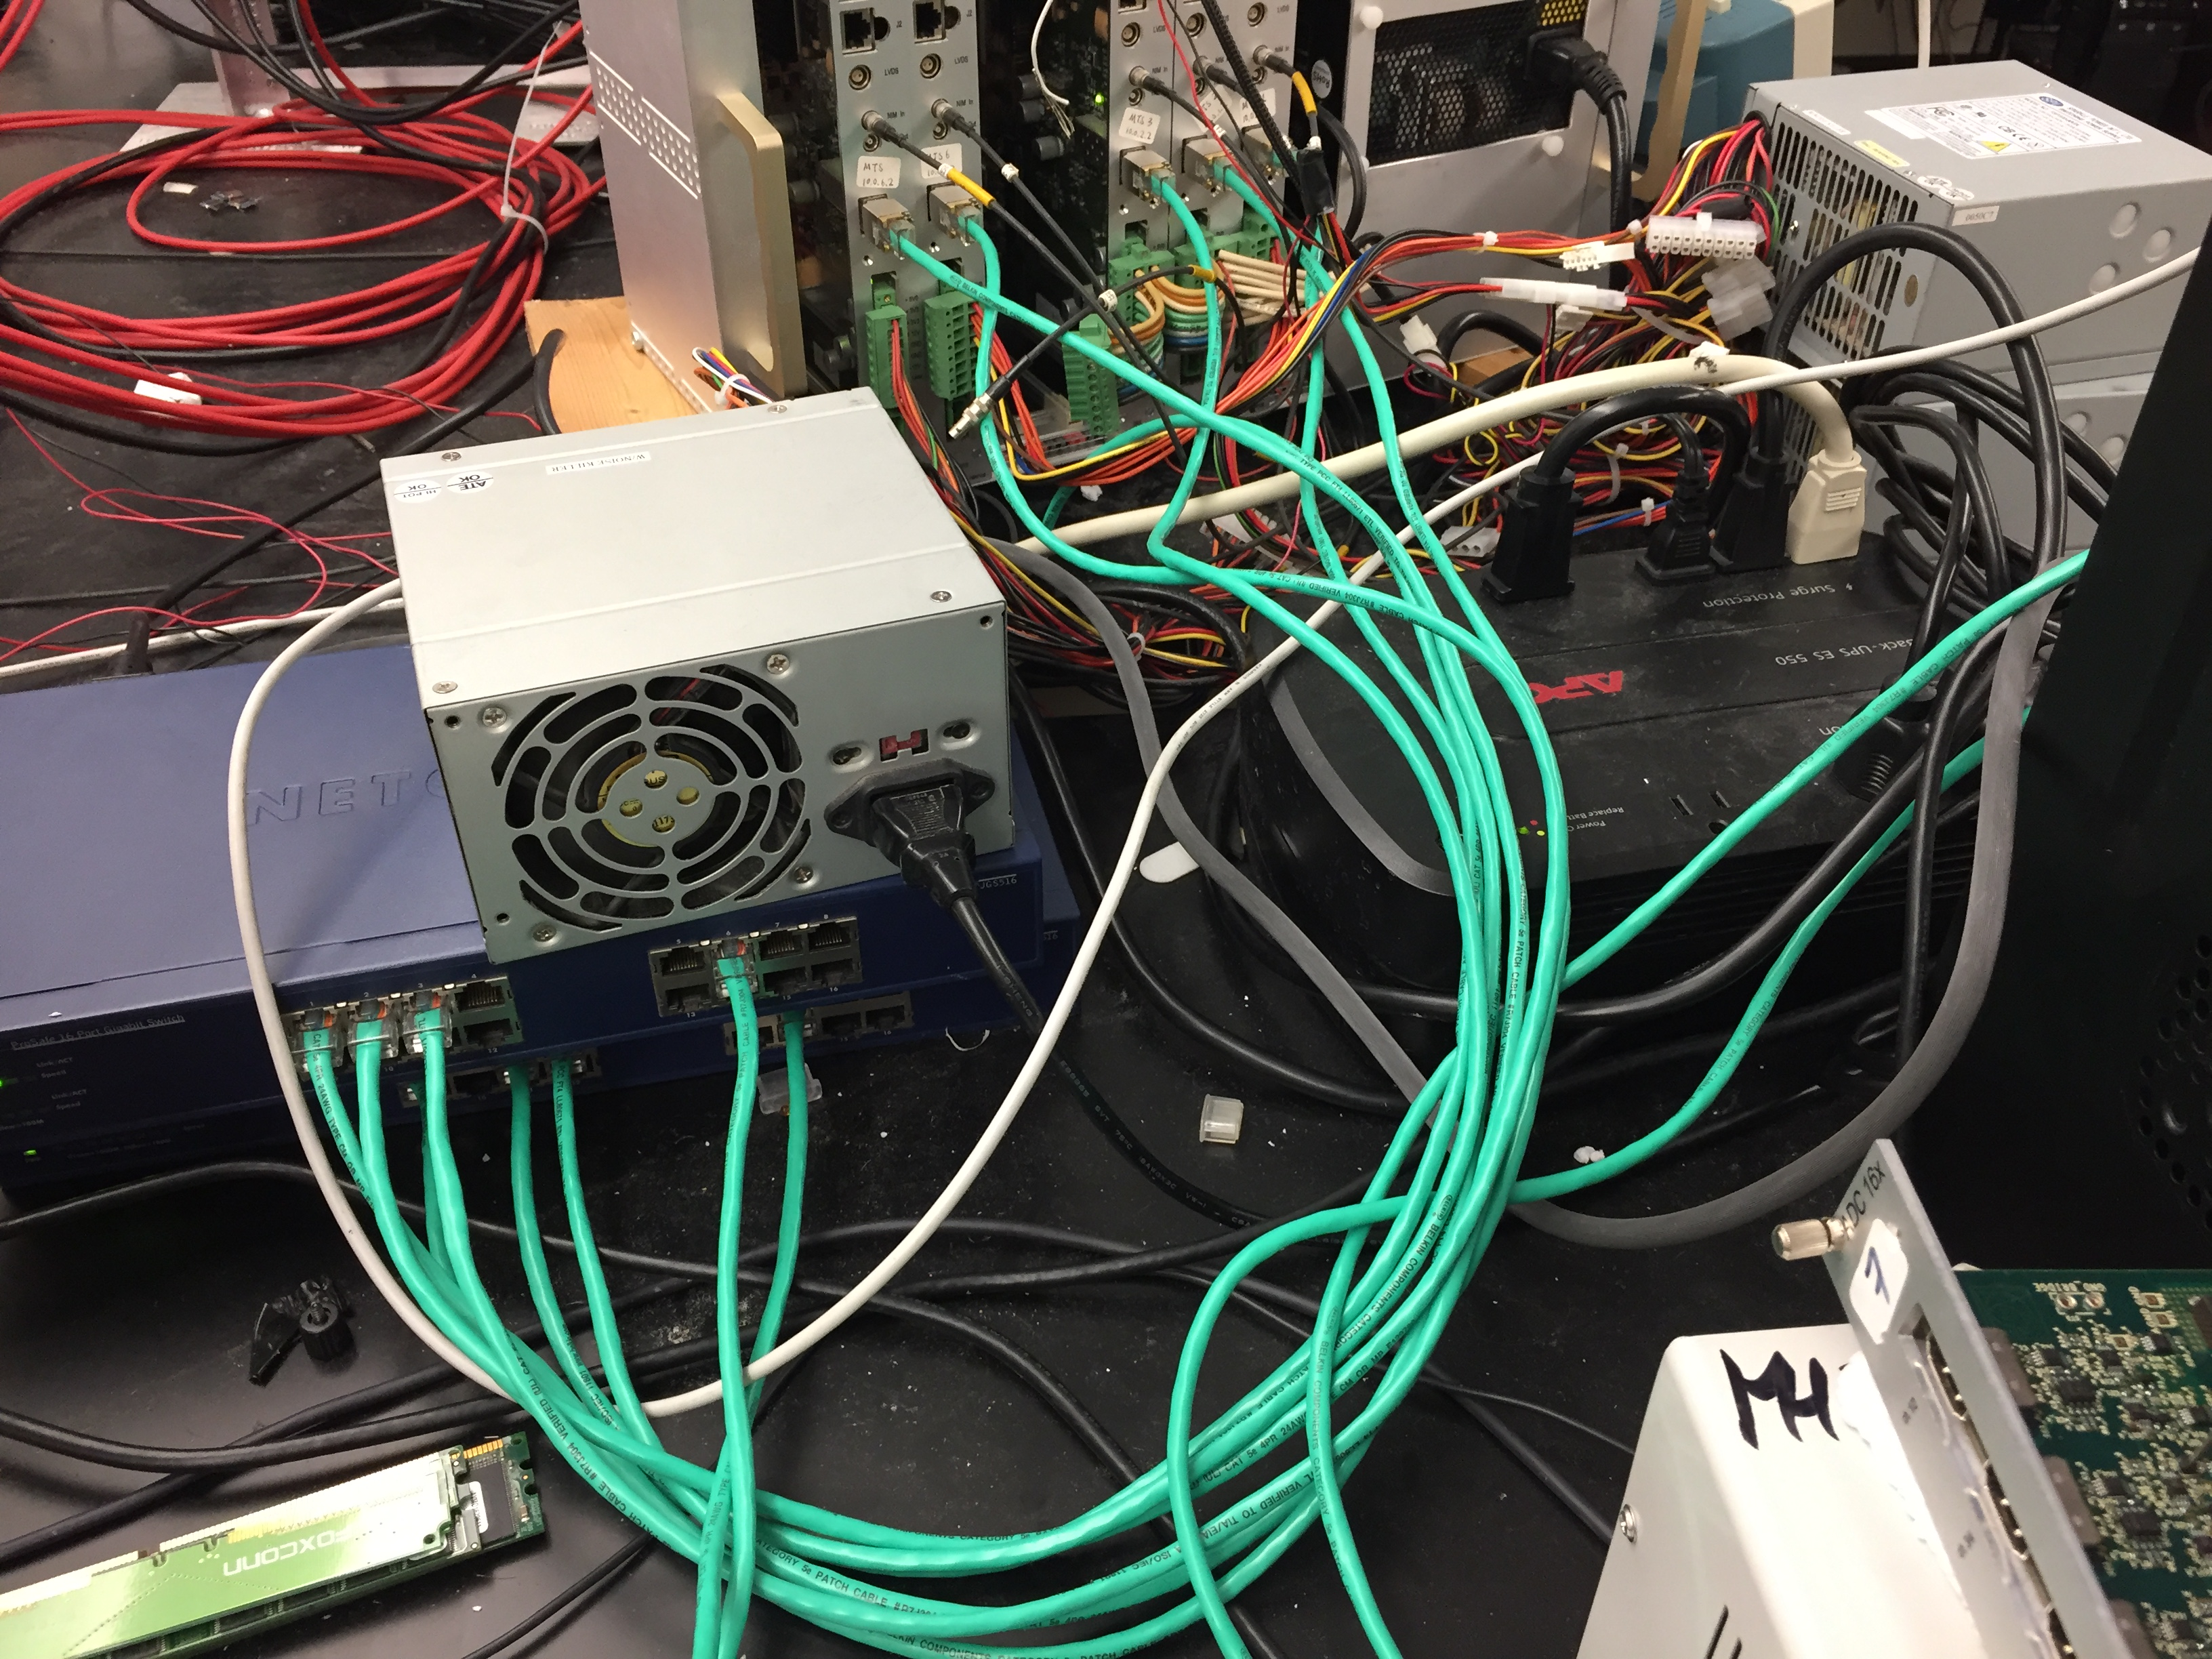
\includegraphics[scale=0.06]{mtsCables.png}}
%  \end{figure}

    \begin{center}
      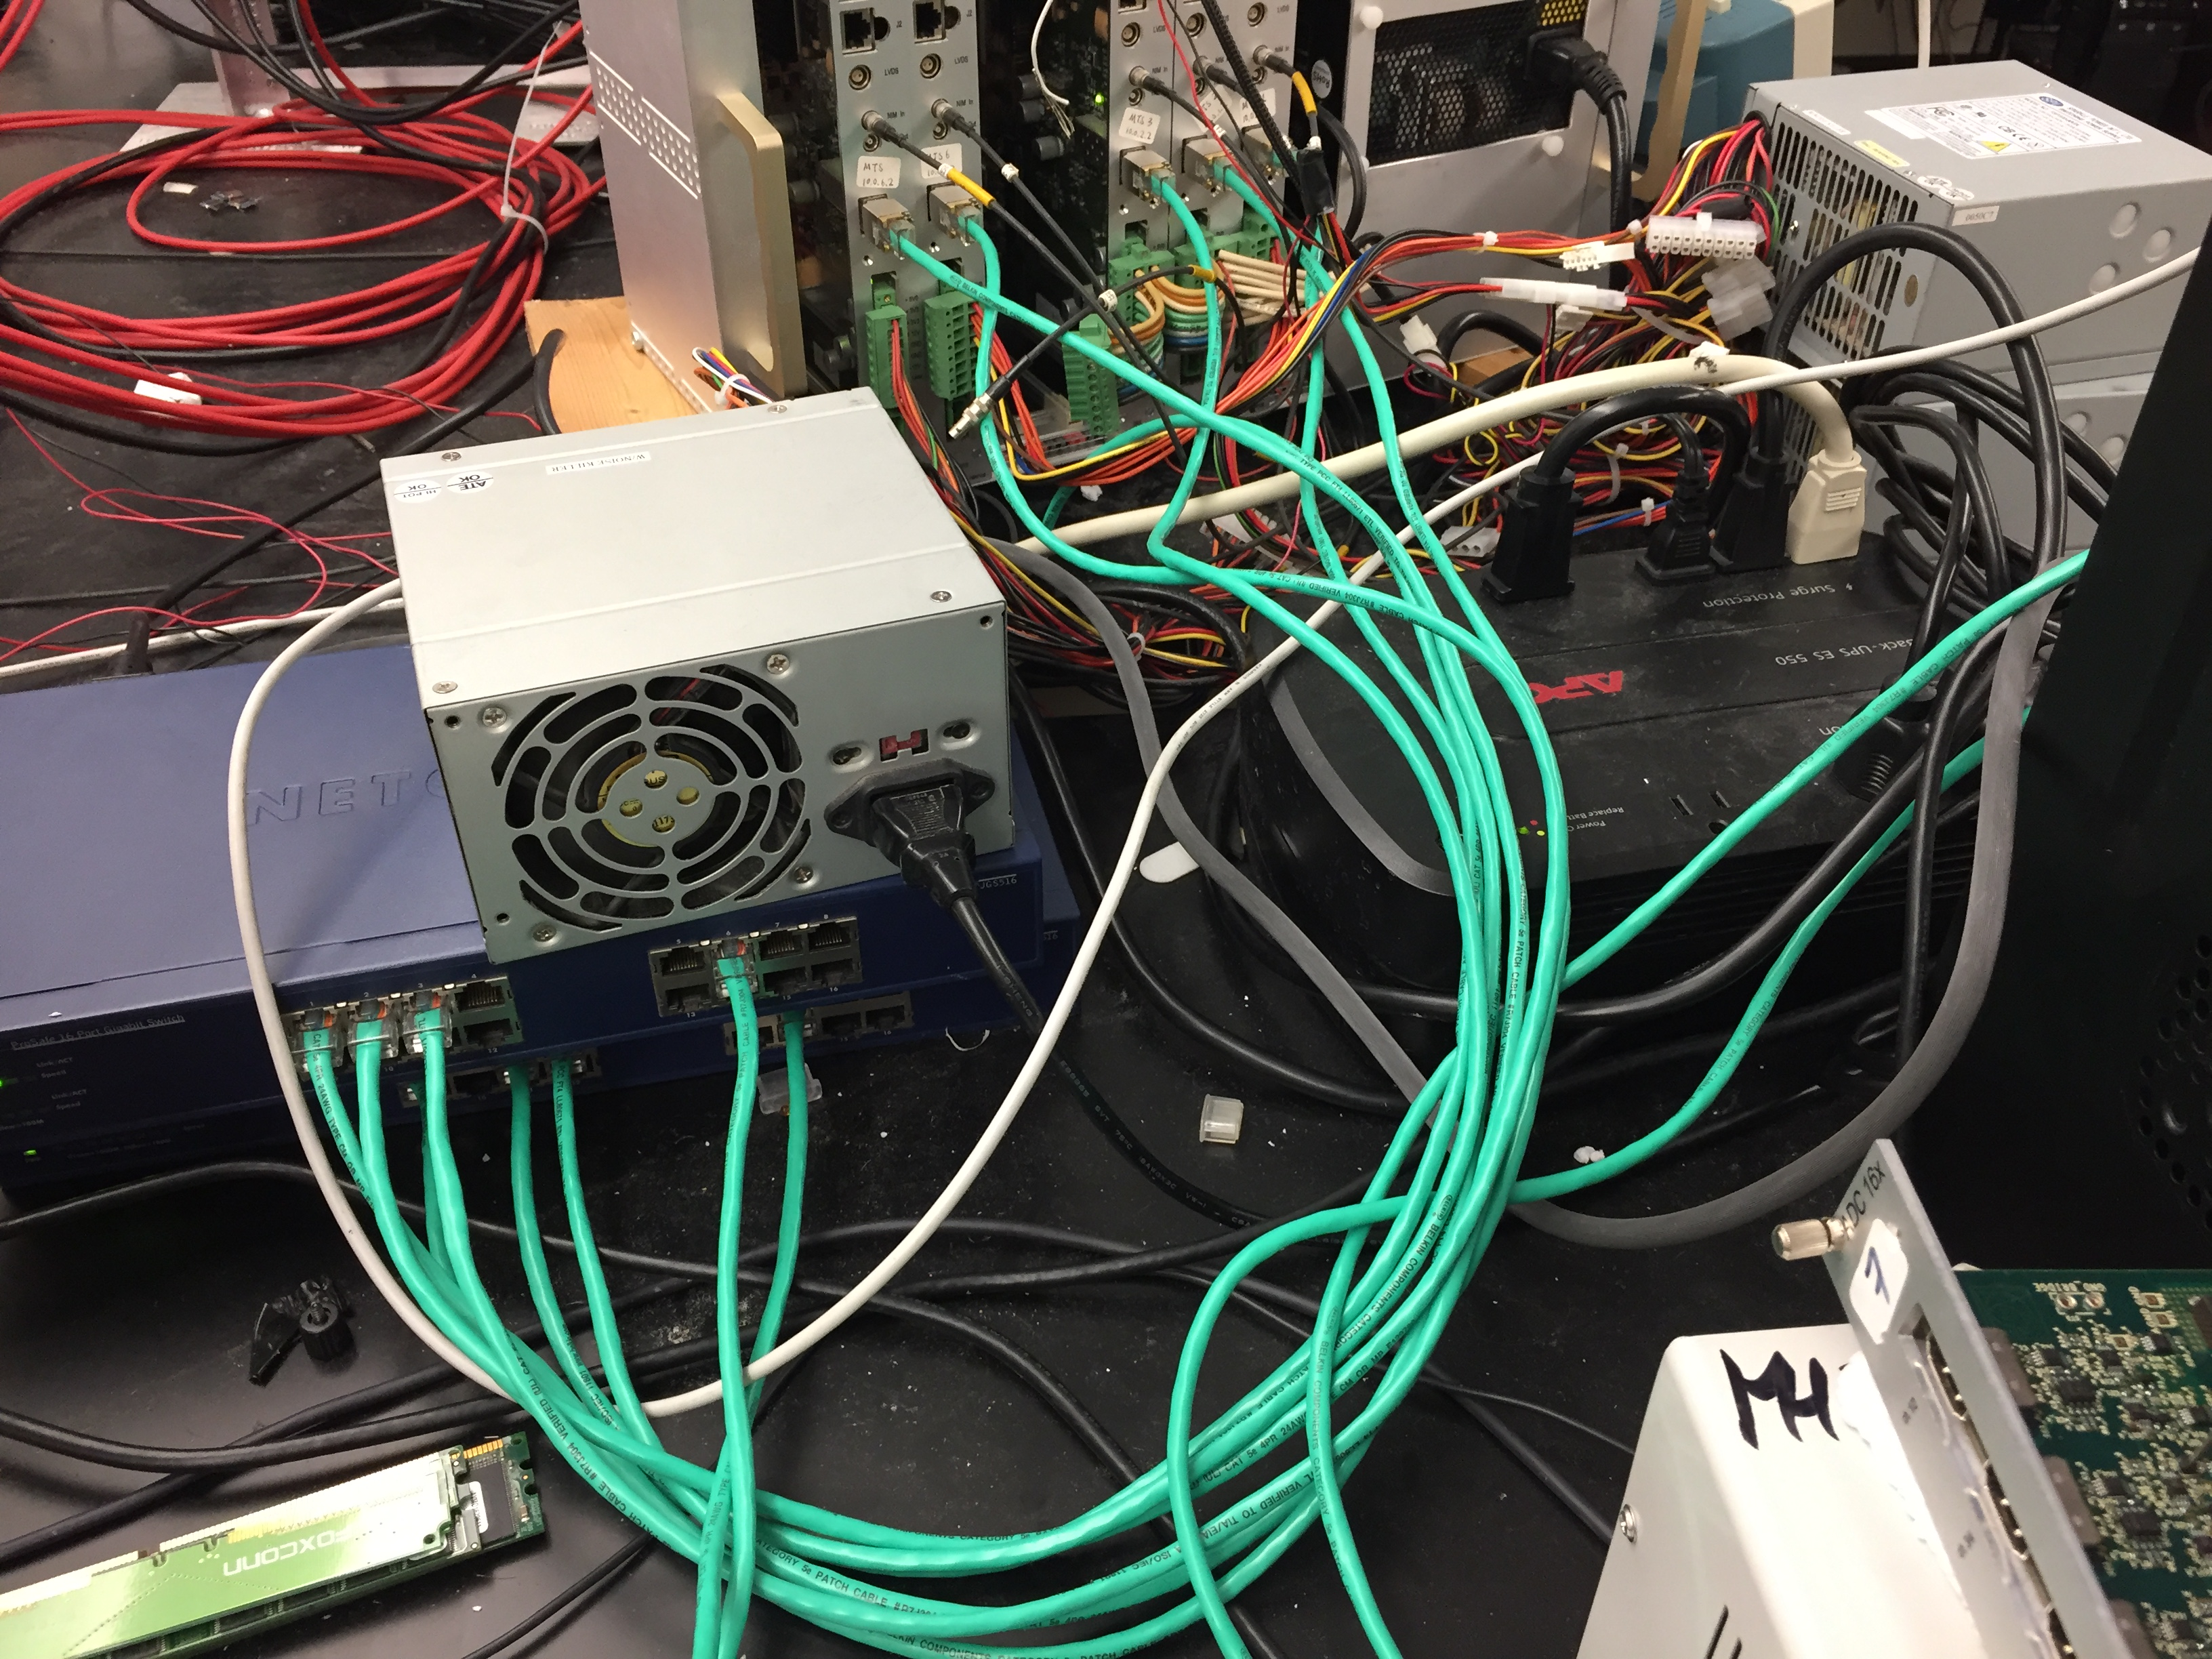
\includegraphics[scale=0.06]{mtsCables.png}
    \end{center}    

\end{frame}

%-----------END EXISTING MTS-----------

%----------BEGIN DEVELOPMENT MTS----------

\subsection{Development MTS}

\begin{frame}

  \frametitle{Development MTS}

  \begin{itemize}
    \item Attempted a reinstall of ROOT and AMORE to help solve issues
    \item Reinstallation of ROOT solved ROOT problems
    \item Tried to reinstall AMORE only to find that its repository has been
      decommissioned and AMORE no longer supported
    \item Fortunately, we are in communication with former lab member who has
      access to the AMORE source on CERN's private GitHub
  \end{itemize}

  \begin{multicols}{2}
    
    \begin{figure}[H]
      \begin{center}
        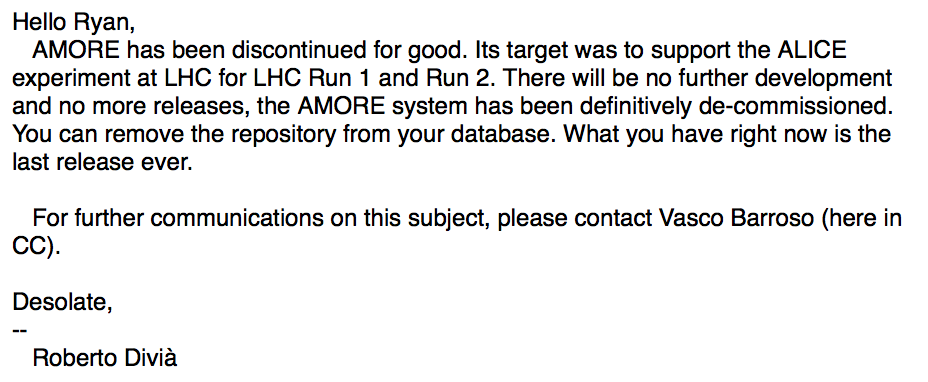
\includegraphics[scale=0.4]{AMOREGoneEmail.png}
      \end{center}
    \end{figure}
    
    \columnbreak

    \begin{figure}[H]
      \begin{center}
        
\includegraphics[scale=0.4]{StefanoEmail.png}
      \end{center}
    \end{figure}

  \end{multicols}

\end{frame}

%-----------END DEVELOPMENT MTS-----------

%----------BEGIN MILESTONE 5 GOALS----------

\section{Milestone 5 Goals}

\begin{frame}

  \frametitle{Milestone 5 Goals}

  \begin{center}
  \begin{tabular}{|c|c|c|c|}
    \hline
    Task & Eric & Josef & Ryan \\
    \hline
    Continue to Care for Existing MTS & 60\% & 20\% & 20\% \\
    Compile Instructions for MTS Operation & 20\% & 40\% & 40\% \\
    Prepare Development MTS Machine & 20\% & 50\% & 30\% \\
    Integrate Nodes into Cluster & 10\% & 10\% & 80\% \\
    Assist Researchers & 70\% & 10\% & 20\% \\
    \hline
  \end{tabular}
\end{center}

\end{frame}

%-----------END MILESTONE 5 GOALS-----------

%----------BEGIN QUESTIONS----------

\section{Questions}

\begin{frame}

  \frametitle{Questions}

  \begin{center}
    {\fontsize{200}{200}\selectfont ?}
  \end{center}
  
\end{frame}

%-----------END QUESTIONS-----------


\end{document}
